\documentclass[brazil]{beamer}
\usepackage[brazilian]{babel}
\usepackage[utf8]{inputenc}
\usepackage{graphics}
\usepackage{listings}
\usepackage{color}
\usetheme{Szeged}
\usecolortheme{whale}

\title{Comparação de eficiência entre OpenCL e CUDA}
\author{Thiago de Gouveia Nunes}

\definecolor{dkgreen}{rgb}{0,0.6,0}
\definecolor{gray}{rgb}{0.5,0.5,0.5}
\definecolor{mauve}{rgb}{0.58,0,0.82}

\lstset{ %
  language={[x86masm]Assembler},                % the language of the code
  basicstyle=\scriptsize,           % the size of the fonts that are used for the code
  numbers=left,                   % where to put the line-numbers
  numberstyle=\tiny\color{gray},  % the style that is used for the line-numbers
  stepnumber=2,                   % the step between two line-numbers. If it's 1, each line 
                                  % will be numbered
  numbersep=5pt,                  % how far the line-numbers are from the code
  backgroundcolor=\color{white},      % choose the background color. You must add \usepackage{color}
  showspaces=false,               % show spaces adding particular underscores
  showstringspaces=false,         % underline spaces within strings
  showtabs=false,                 % show tabs within strings adding particular underscores
  frame=single,                   % adds a frame around the code
  rulecolor=\color{black},        % if not set, the frame-color may be changed on line-breaks within not-black text (e.g. comments (green here))
  tabsize=2,                      % sets default tabsize to 2 spaces
  captionpos=b,                   % sets the caption-position to bottom
  breaklines=true,                % sets automatic line breaking
  breakatwhitespace=false,        % sets if automatic breaks should only happen at whitespace
  title=\lstname,                   % show the filename of files included with \lstinputlisting;
                                  % also try caption instead of title
  keywordstyle=\color{blue},          % keyword style
  commentstyle=\color{dkgreen},       % comment style
  stringstyle=\color{mauve},         % string literal style
  escapeinside={\%*}{*)},            % if you want to add LaTeX within your code
  morekeywords={*,...},              % if you want to add more keywords to the set
  deletekeywords={...}              % if you want to delete keywords from the given language
}

\begin{document}

\frame{\titlepage}

%-------------------------------------
\section{Tecnologias}
%-------------------------------------

\frame{
  \frametitle{GPGPU}
  O que é GPGPU?
}

\frame{
  \frametitle{GPGPU}
  Existem 2 linguagens populares no mercado para GPGPU, o \textbf{CUDA} (Compute Unified Device Architecture) feita pela
  \textit{NVIDIA}, e o \textbf{OpenCL} (Open Computing Language), iniciativa open source de um conjunto de empresas.
}

\frame{
  \frametitle{OpenCL}
    \begin{columns}
      \begin{column}{.5\textwidth}
        
\includegraphics[scale=0.7]{OpenCL_Logo.png}
      \end{column}
      \begin{column}{.5\textwidth}
         O OpenCL é uma linguagem de programação paralela para sistemas híbridos. Atualmente o OpenCL está na versão 1.2.
      \end{column}
    \end{columns}
}

\frame{
  \frametitle{CUDA}
  \begin{columns}
    \begin{column}{.5\textwidth}
      
\includegraphics[scale=0.3]{CUDAlogo.jpg}
    \end{column}
    \begin{column}{.5\textwidth}
      CUDA é uma linguagem proprietária para programação paralela em GPUs desenvolvida pela NVIDIA. O CUDA está na versão 5.0 atualmente.
    \end{column}
  \end{columns}
  
}

\begin{frame}[fragile]
  \frametitle{Como comparar?}
  Bem, para comparar as linguagens, vamos observar 2 aspectos delas:
  \begin{enumerate}
    \item Taxa de acesso a memória;
    \item Mêtodo de execução.
  \end{enumerate}
  Para entender o impacto desses aspectos no tempo de execução, vamos dar uma olhada no hardware de uma GPU...
\end{frame}

\frame{
  \frametitle{GPU}
  \begin{columns}
    \begin{column}{.6\textwidth}
  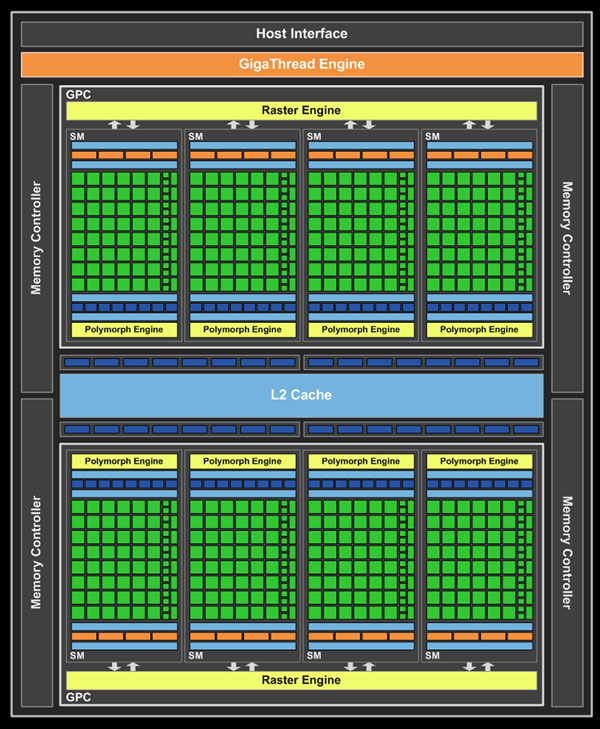
\includegraphics[scale=0.28]{15596_large_GTX460_Architecture.jpg}  
    \end{column}
    \begin{column}{.4\textwidth}
      Representação do hardware de uma GTX 460 SE da NVIDIA.
    \end{column}
  \end{columns}
}

\begin{frame}[fragile]
  \frametitle{Arquitetura GeForce GTX 460 SE}
  \begin{columns}
    \begin{column}{.5\textwidth}
      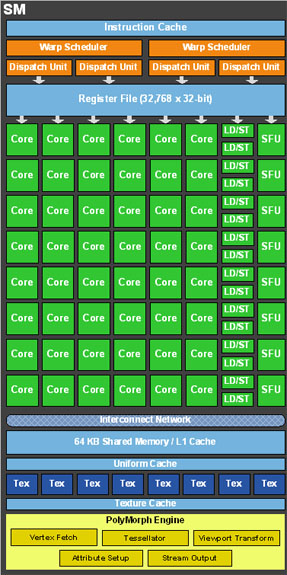
\includegraphics[scale=0.35]{embed-arch2.jpg}  
    \end{column}
    \begin{column}{.5\textwidth}
      A GPU é subdividida em vários Streaming Multiprocessor, como o do lado, que agrupam 48 processadores.
    \end{column}
  \end{columns}
\end{frame}

\begin{frame}[fragile]
  \frametitle{Como um programa roda na GPU?}
  \begin{columns}
    \begin{column}{.4\textwidth}
      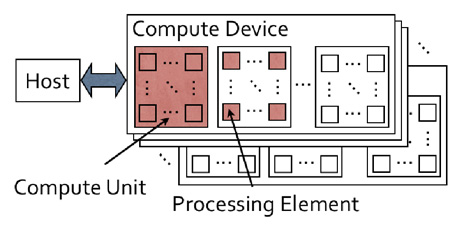
\includegraphics[scale=0.3]{opencl_figure2small.jpg}
    \end{column}
    \begin{column}{.6\textwidth}
      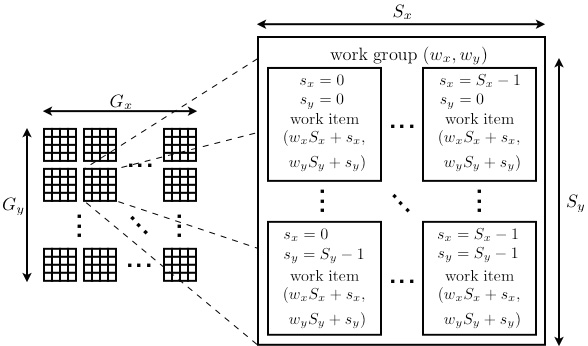
\includegraphics[scale=0.3]{opencl_figure3.jpg}
    \end{column}
  \end{columns}
\end{frame}

%-------------------------------------
\section{Comparação entre as linguagens}
%-------------------------------------

\frame{
  \frametitle{Semelhanças}
  Alguns elementos são iguais para as duas linguagens.
  \begin{itemize}
    \item Para iniciar a execução num device é necessario que um programa chamado de host inicie o ambiente de execução na GPU.
    \item As threads executando no device são identificadas por indices.
    \item As threads são agrupadas em conjuntos antes de serem enviadas para execução no device.
    \item A alocação e preenchimento da memória no device é controlada pelo host.
    \item A execução dos kernels pode ser síncrona ou assíncrona com o a execução do host.
  \end{itemize}
}

\frame{
  \frametitle{Semelhanças}
  \begin{itemize}
      \item Existem 4 locais diferentes para a memória que é enviada para o device:
        \begin{enumerate}
         \item Global Memory  - Toda e qualquer thread tem acesso a essa memória.
         \item Constat Memory - Memória que permanece fixa ao andar da execução.
         \item Local Memory   - Região da memória dividida pelas threads de um mesmo SM.   
         \item Private Memory - Região privada para cada thread.
       \end{enumerate} 
  \end{itemize}
}

\frame{
  \frametitle{Diferenças - Plataforma}
  No OpenCL existem 2 tipos de execução diferentes:
  \begin{enumerate}
    \item Data Parallel
    \item Task Parallel
  \end{enumerate}
  O CUDA implementa o modelo SIMT (\textit{Single Instruction, Multiple Thread}).
}

%-------------------------------------
\section{Comparação de Performance}
%-------------------------------------

\frame{
  \frametitle{Ideia}
  Para comparar a performance das duas linguagens foram usados dois tipos de kernel, um em que o desempenho está ligado ao acesso a
  memória (memory bound) e outro que está ligado à velocidade de processamento (compute bound).
}

\frame{
  \frametitle{Kernel Memory bound} 
  Para comparar o acesso a memória, foi usado um kernel que faz a cópia de uma matriz de floats para outras.
} 

\begin{frame}[fragile]
  \frametitle{Kernel Memory Bound}
  \begin{lstlisting}
    __kernel void matrixmulti(__global float* a, 
          __global float* b, 
          __global int* rowSize, 
          __global int* columnSize) {
          
      unsigned int row = get_global_id(0);
      unsigned int column = get_global_id(1);
      
      b[row+column*(*rowSize)] 
          = a[row+column*(*rowSize)];
    }
  \end{lstlisting}
\end{frame}

\frame{
  \frametitle{Kernel Compute bound}
  Para comparar o processamento, um kernel que multiplica duas matrizes de doubles e guarda o valor numa terceira fui usado.
}

\begin{frame}[fragile]
  \frametitle{Kernel Compute bound}
  \begin{lstlisting}
    __kernel void matrixmulti(__global int* a, 
                              __global int* b, 
                              __global int* c, 
                              __global int* size) {
        unsigned row = get_global_id(0);
        unsigned column = get_global_id(1);
        unsigned i;
        
        row *= (*size);
        c[row+column] = 0;
        for( i = 0; i < (*size); i++ ) 
            c[row+column] += 
                a[row+i]*b[i*(*size)+column];
    }
  \end{lstlisting}
\end{frame}

\begin{frame}[fragile]
  \frametitle{Estatistica Memory bound}
  \begin{columns}
    \begin{column}{.5\textwidth}
      \begin{figure}
          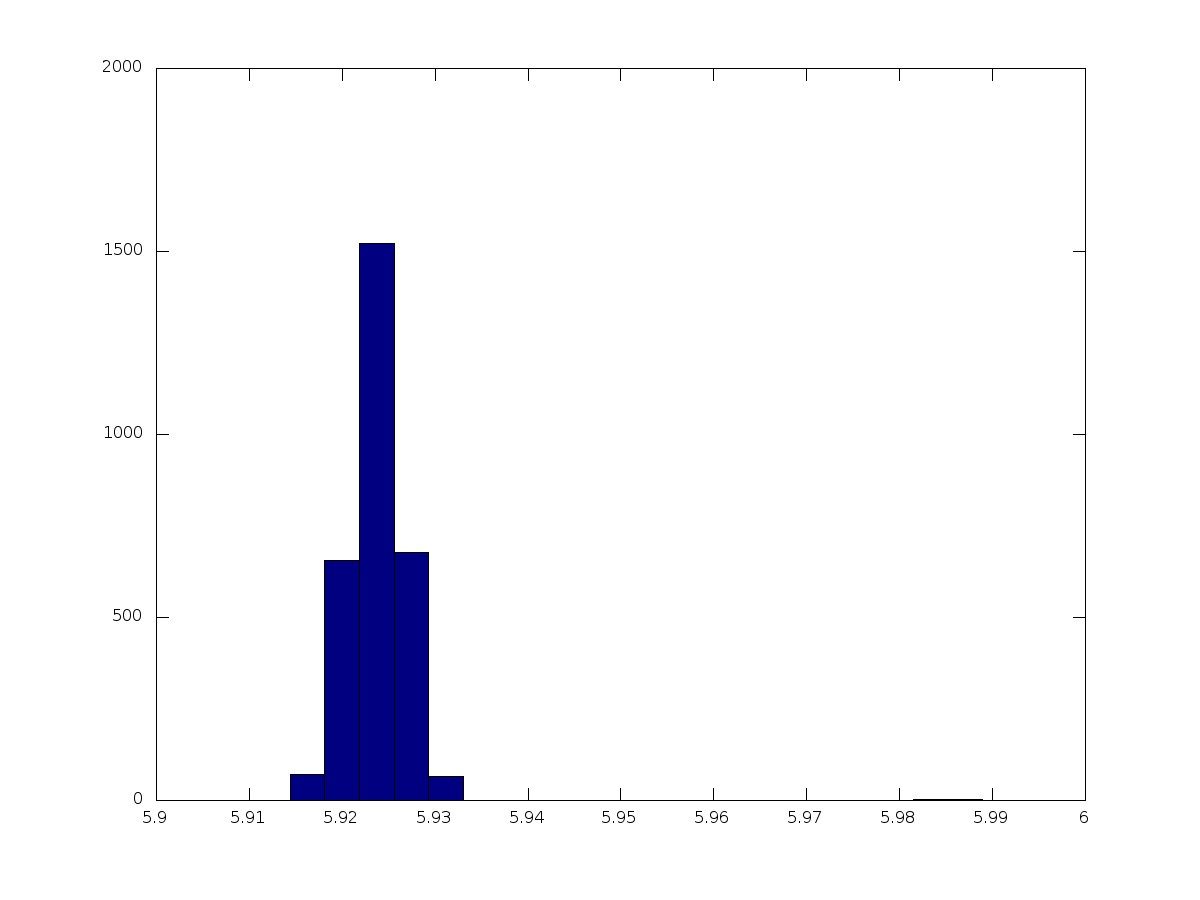
\includegraphics[scale=0.15]{resultados_cuda_memory_histo.jpg} \\
          CUDA
      \end{figure}
    \end{column}
    \begin{column}{.5\textwidth}
      \begin{figure}
          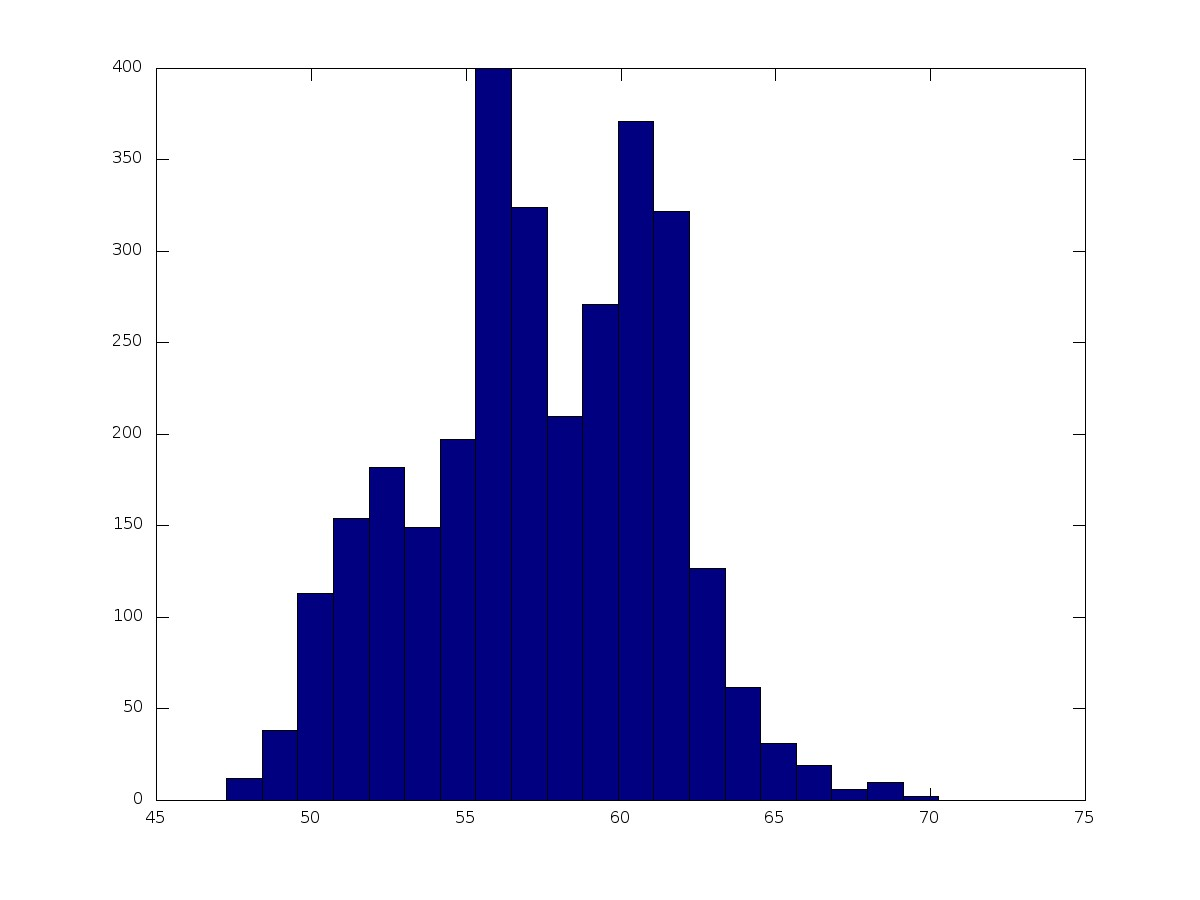
\includegraphics[scale=0.15]{resultados_opencl_memory_histo.jpg} \\
          OpenCL
      \end{figure}
    \end{column}
  \end{columns}
\end{frame}

\begin{frame}[fragile]
  \frametitle{Estatistica Process bound}
  \begin{columns}
    \begin{column}{.5\textwidth}
      \begin{figure}
          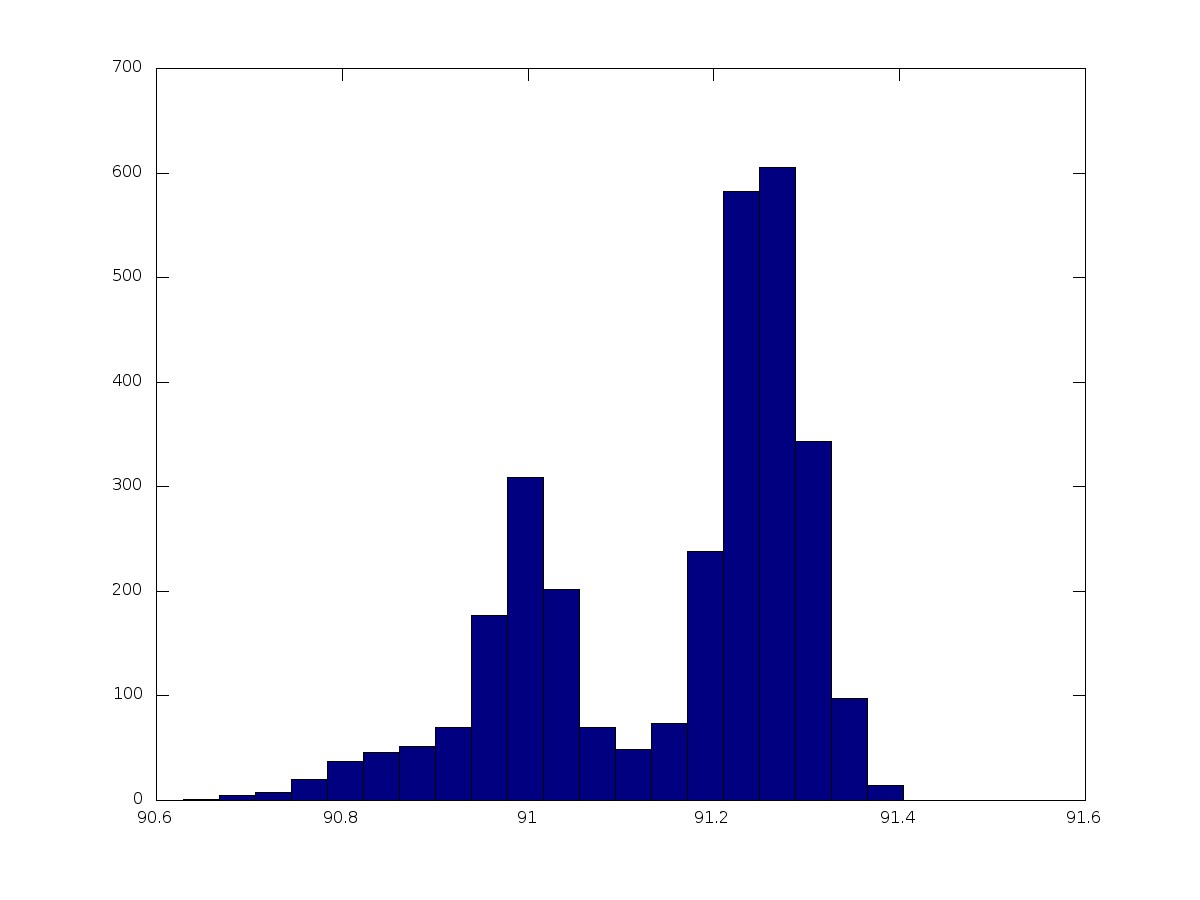
\includegraphics[scale=0.15]{resultados_cuda_process_histo.jpg} \\
          CUDA        
      \end{figure}
    \end{column}
    \begin{column}{.5\textwidth}
      \begin{figure}
          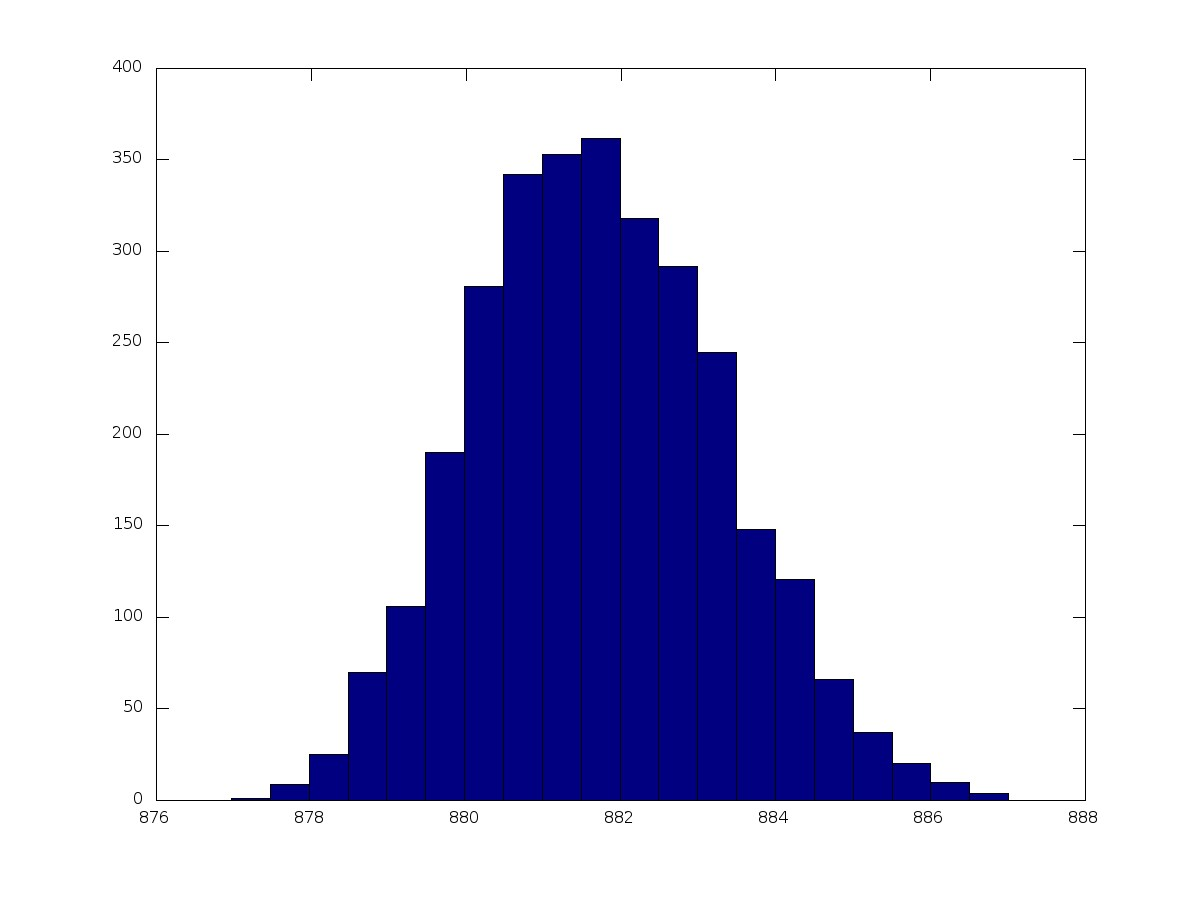
\includegraphics[scale=0.15]{resultados_opencl_process_histo.jpg} \\
          OpenCL
      \end{figure}
    \end{column}
  \end{columns}
\end{frame}

\frame{
  \frametitle{Explicação dos PTX}
  Para melhorar a compatibilidade dos programas rodando em GPUs diferentes, 
  a NVIDIA implementou uma máquina virtual, a Parallel Thread Execution (PTX). 
}

\begin{frame}[fragile]
  \frametitle{Arquivo .ptx}
  \begin{columns}
    \begin{column}{.6\textwidth}
      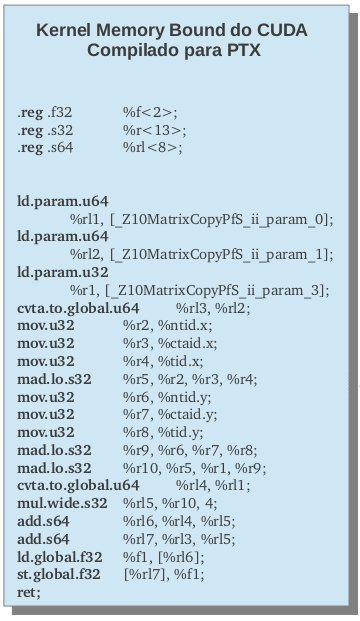
\includegraphics[scale=0.3]{MemBoCuda.jpg}
    \end{column}
    \begin{column}{.5\textwidth}
      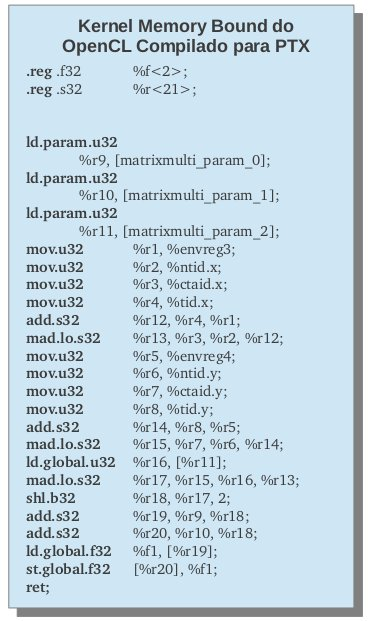
\includegraphics[scale=0.3]{MemBoOpcl.jpg}
    \end{column}
  \end{columns}
\end{frame}

\begin{frame}[fragile]
  \frametitle{Comparação dos PTX}
  Pelos .ptx é possível verificar algumas das diferenças entre as abstrações das linguagens:
  \begin{enumerate}
    \item O OpenCL usa um registrador a mais que o CUDA para calcular o indice de uma thread.
    \item O OpenCL faz mais leituras da memória padrão que o CUDA. 
    \item O OpenCL não tem acesso a todos os comandos do PTX.
  \end{enumerate}
\end{frame}

\begin{frame}[fragile]
  \frametitle{Conclusões}
    O CUDA é mais rápido que o OpenCL em GPUs NVIDIA...
\end{frame}

\end{document}
